\documentclass{report}

\usepackage[english]{babel}
\usepackage[T1]{fontenc}
\usepackage[utf8]{inputenc}

\usepackage[pdfborder={0 0 0}]{hyperref}
\usepackage{graphicx}
\usepackage{array}
\usepackage{tabulary}
\usepackage[top=1.5cm, bottom=1.5cm, left=1.5cm, right=1.5cm]{geometry}
\usepackage{tikz}
\usepackage{menukeys}
\usepackage{multicol}
\usepackage{animate}

\newcolumntype{M}{>{\centering\arraybackslash}m{\dimexpr.25\linewidth-2\tabcolsep}}

\title{Lorann-Ex}
\author{Baptiste Saclier\and Maire Chiaverini\and Clément Chabrier\and Maxime Zupka}
\date{Mercredi 23 Juin 2016}

\begin{document}

\maketitle

\tableofcontents
\clearpage

\chapter{Planning}

At the beginning of the project we had to organize all the project to give differents tasks to the members of the team.

\section{Team}

The team is composed of four persons each have a specific task in the project.

\begin{description}
\item[Baptiste Saclier] \emph{Project leader} : In charge of the organisation of the project and the controller of the software
\item[Marie Chiaverini] In charge of the model of the game, loading systems and data storage
\item[Clément Chabrier] In charge of the view of the project, UML redactor and documentation master
\item[Maxime Zupka] In charge of the design of the level, the documentation and the administration of the database.
\end{description}

\section{Planning diagram}

\subsection{Estimated planning}

\begin{center}
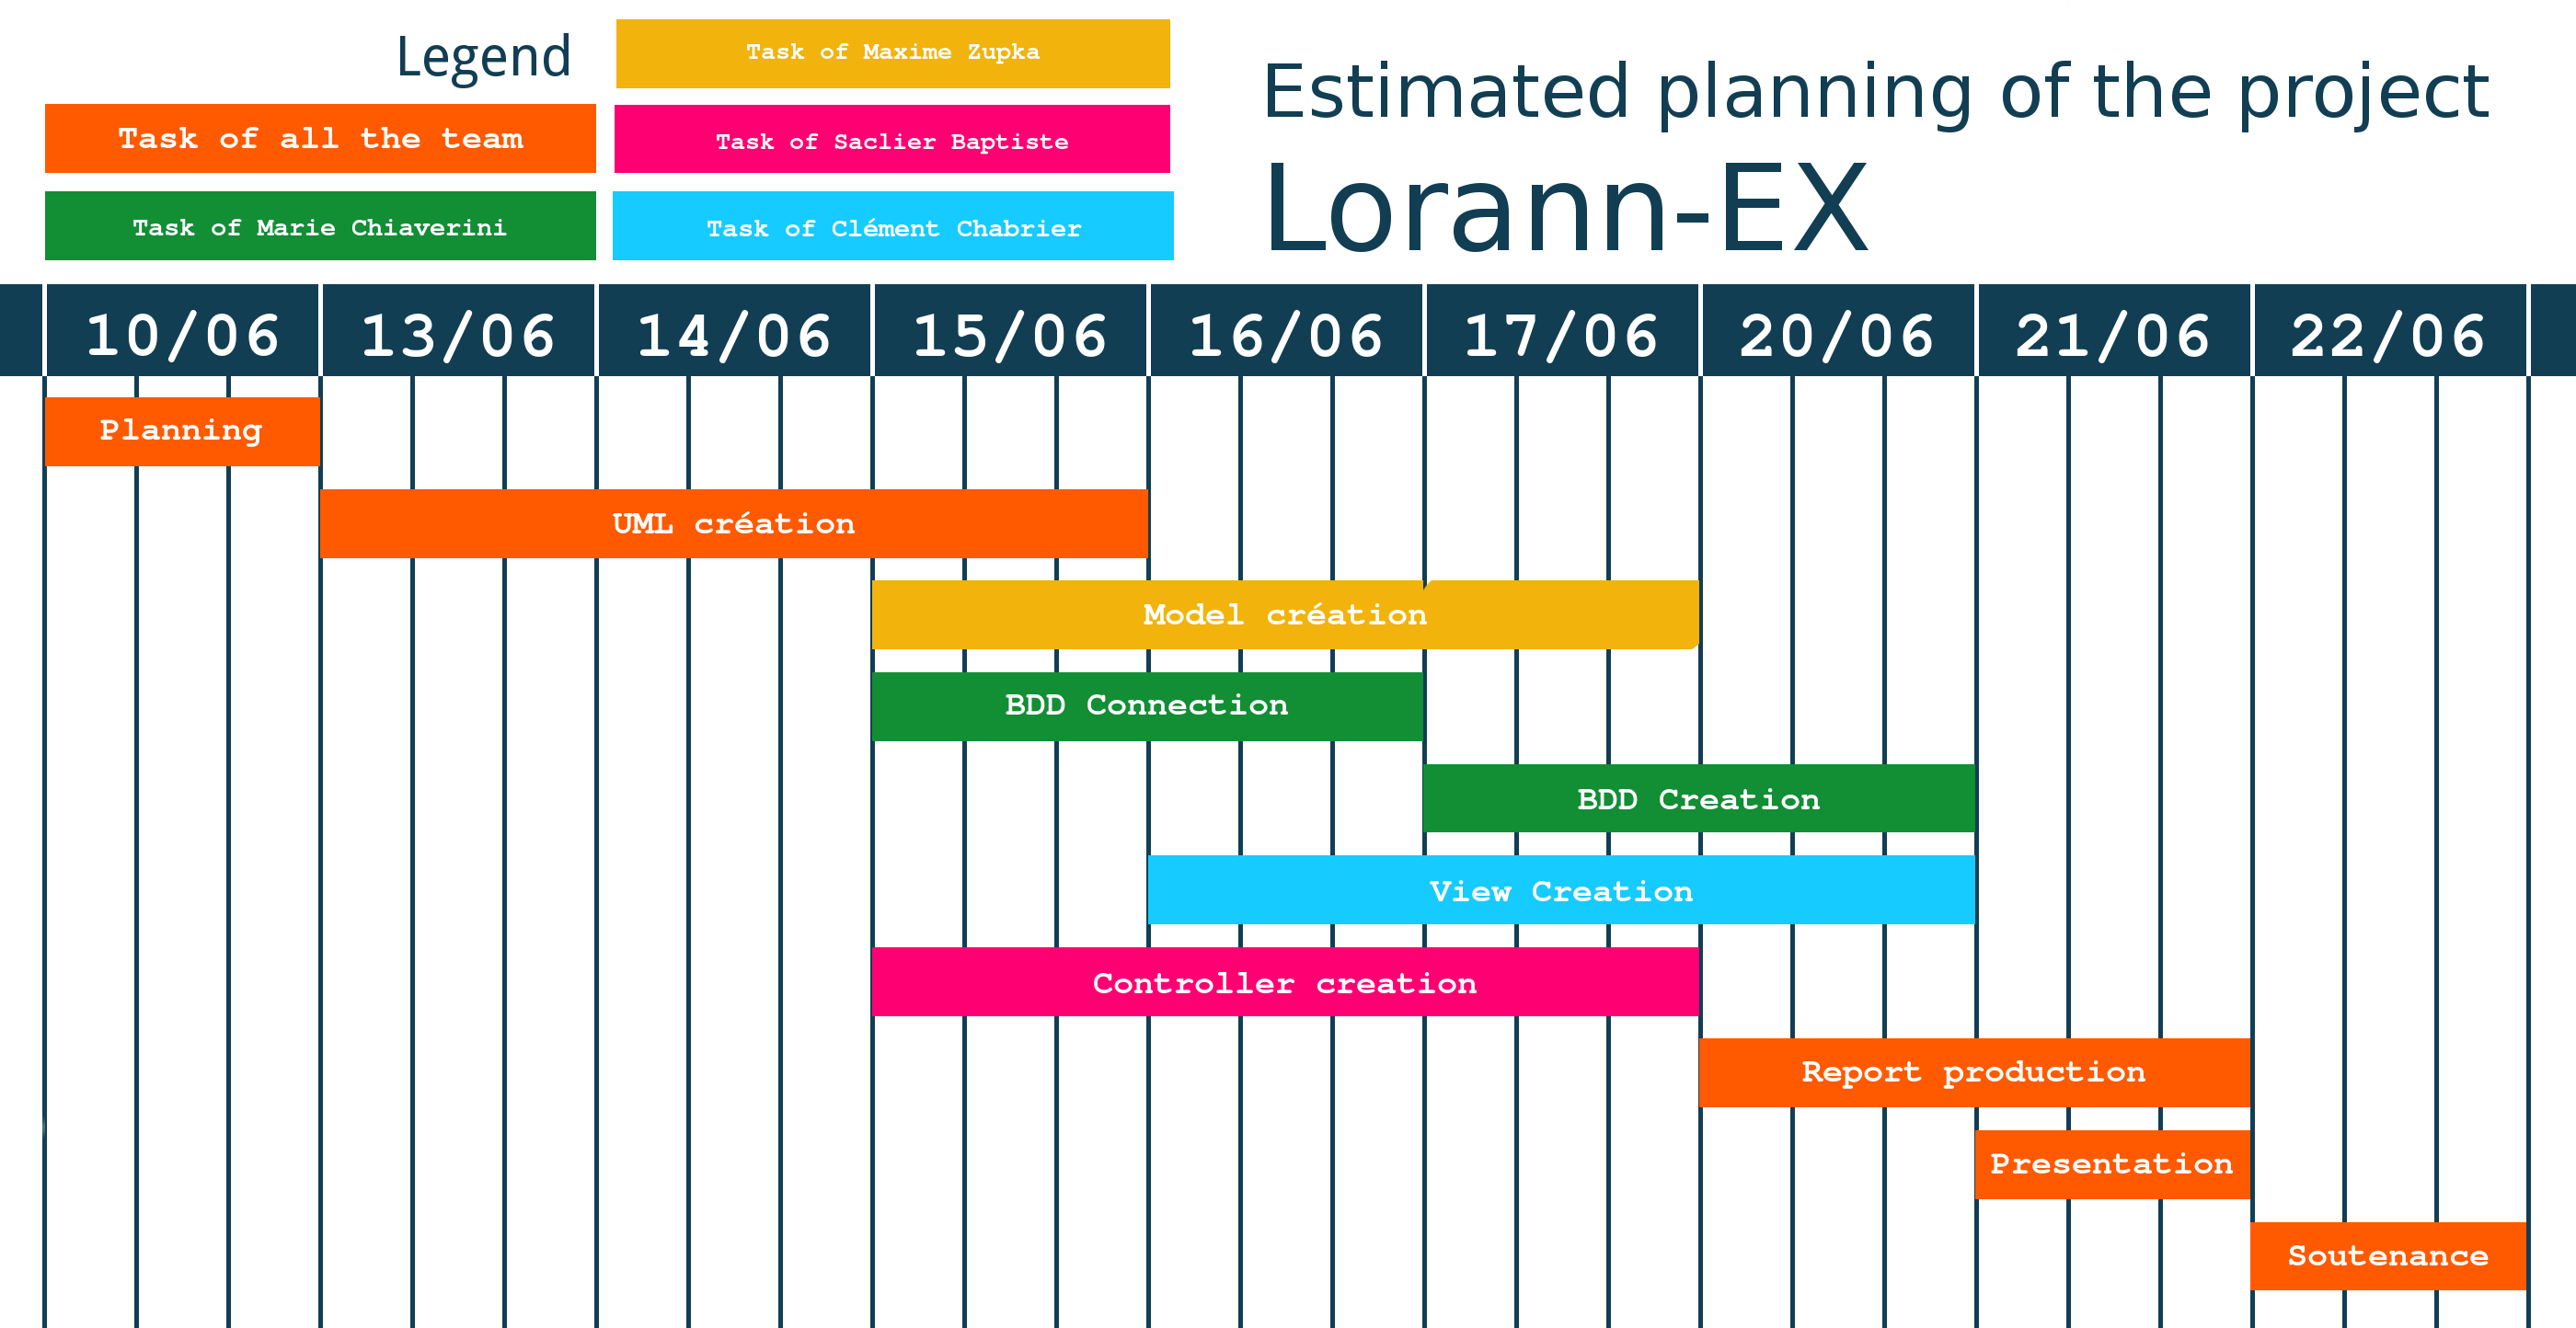
\includegraphics[scale=0.75]{resources/Planning-previsionnel.png}
\end{center}

\subsection{Efficient planning}

\begin{center}
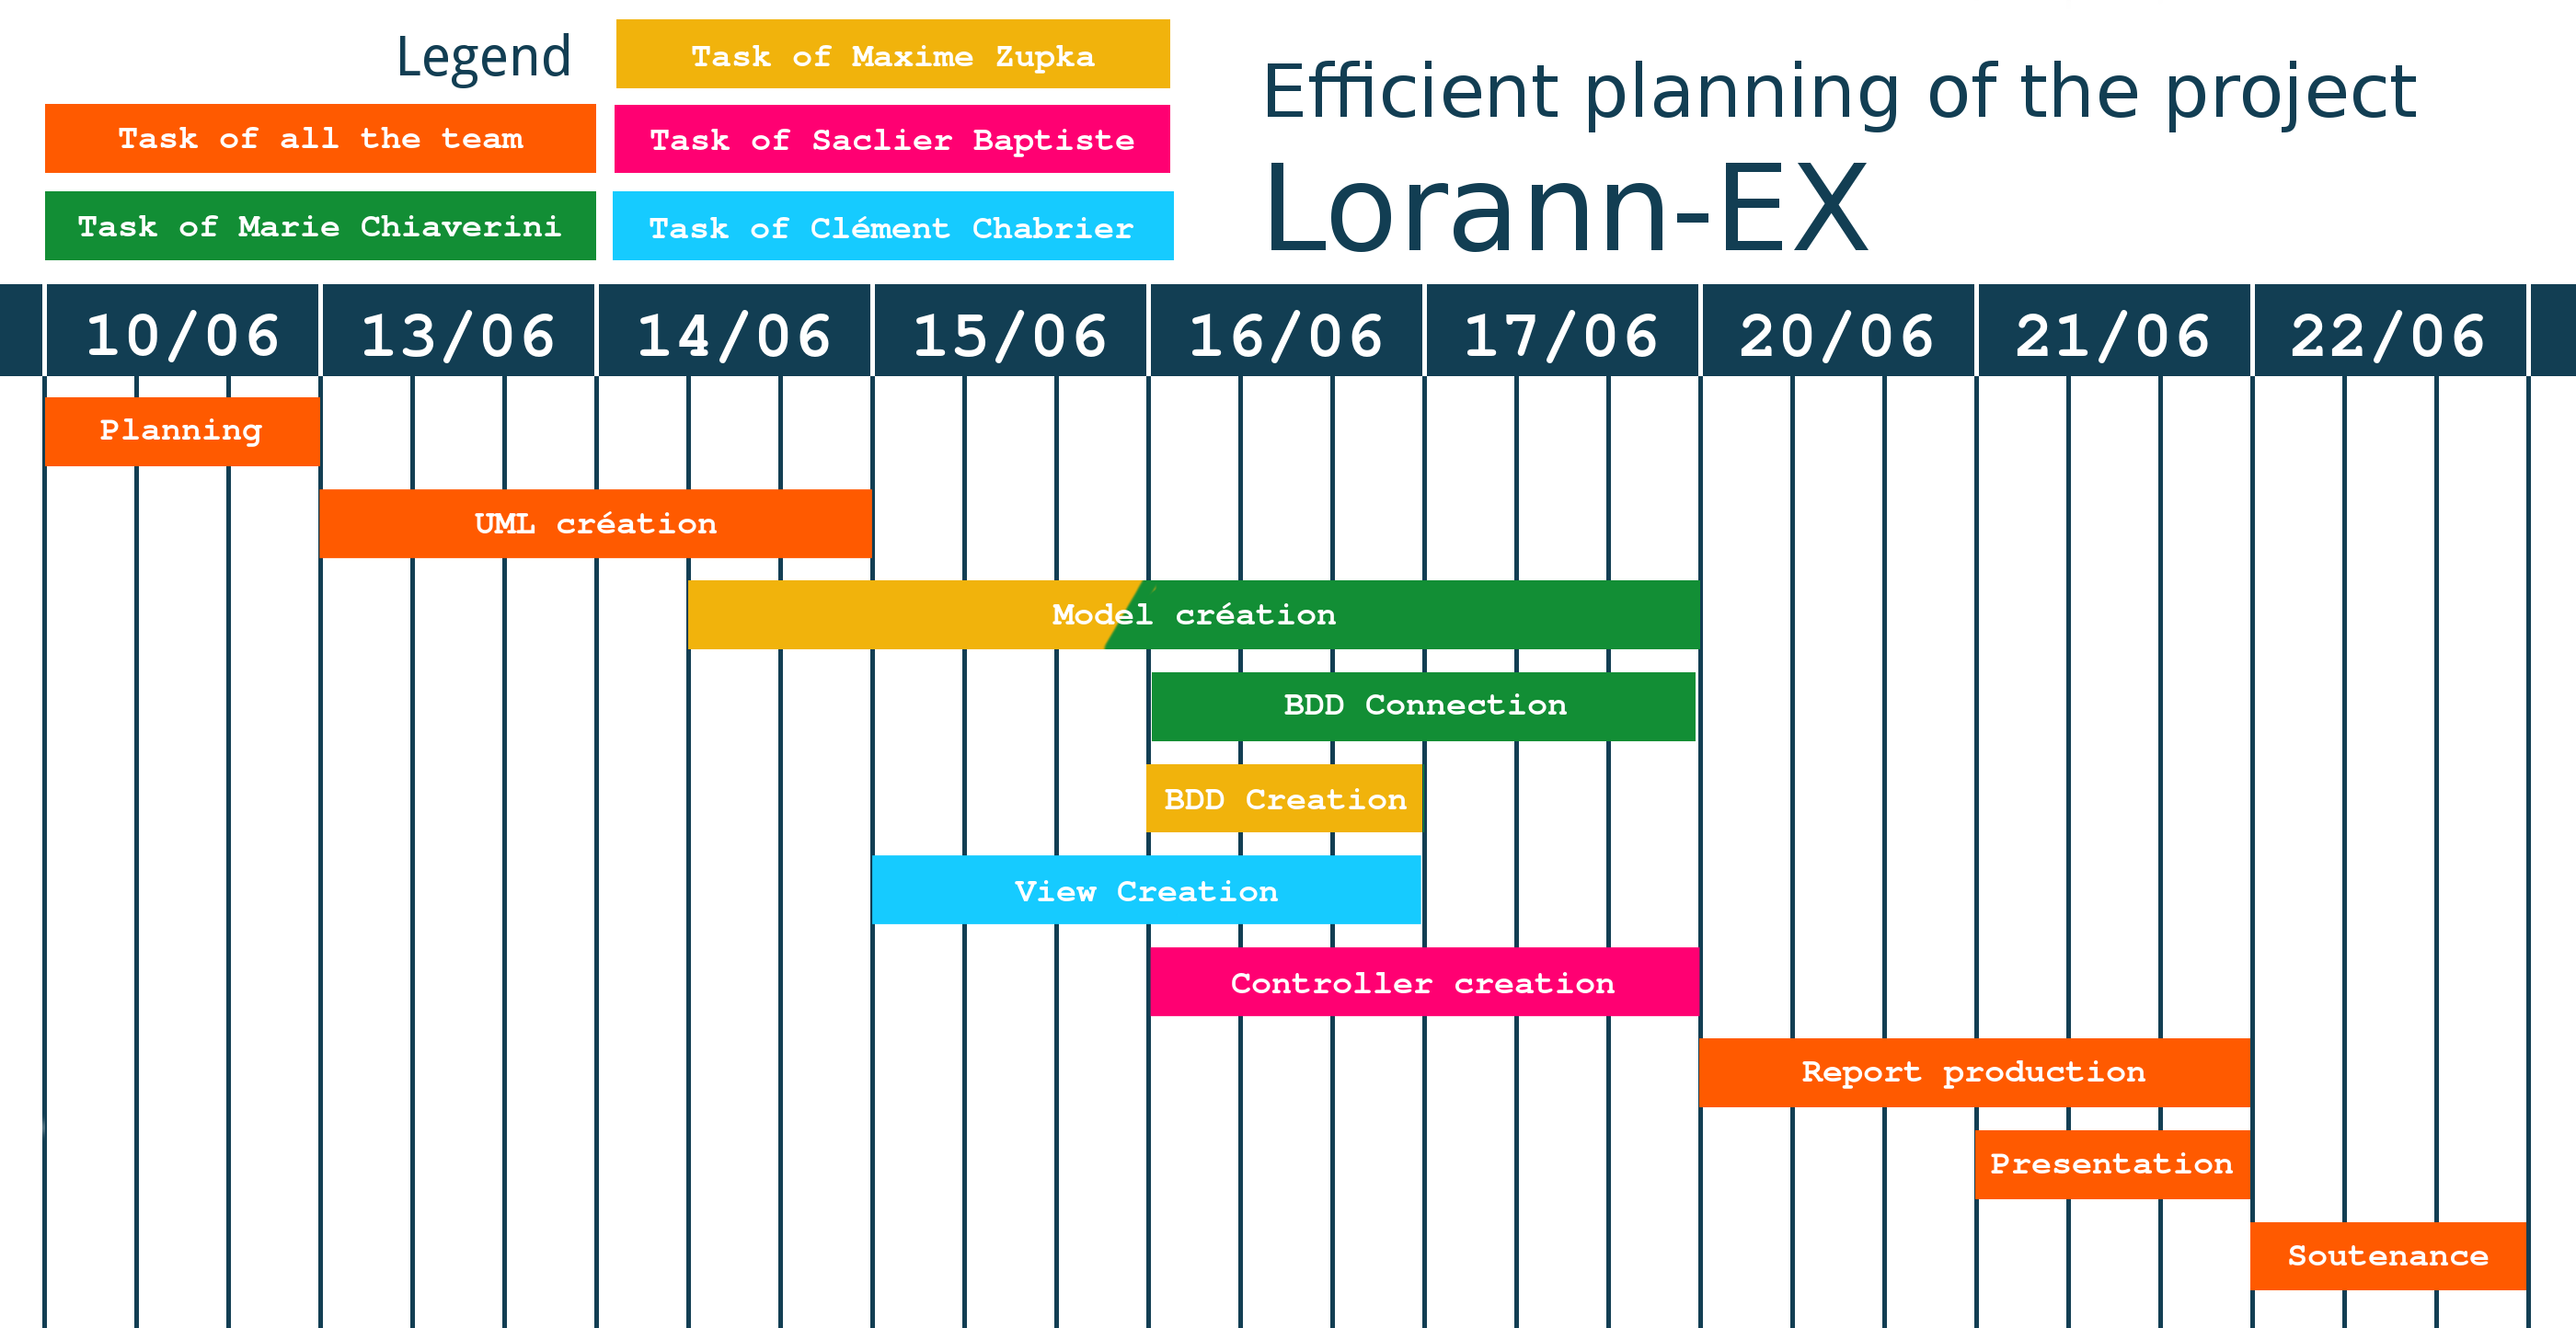
\includegraphics[scale=0.75]{resources/Planning-effectif.png}
\end{center}

\chapter{Game manual}

Welcome to the world of Lorann. In this dungeon you will discover a whole universe of danger in the maze of Nova-Ann. You have to finish all the levels to win the game.

Good luck Lorann.

\section{Installation}

The installation of the game is pretty easy. Just download the executable \emph{JAR} from \emph{github.com} at the address \texttt{\href{https://github.com/EpicKiwi/Lorann-Ex/releases/download/0.0.2/Lorann-Ex-0.0.2-SNAPSHOT.jar}{goo.gl/Mf4zIH}}. And play. The database is distant and fully configurated.

\section{Level}

\begin{center}
\textsf{The first level of the game}\par
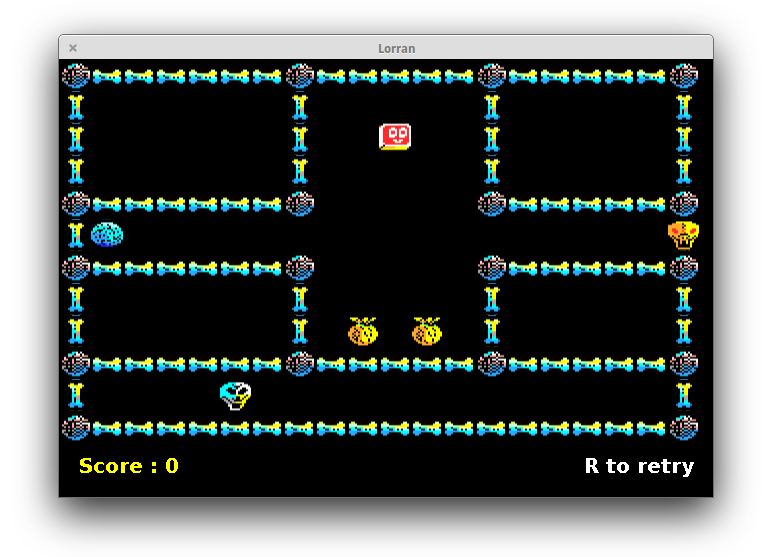
\includegraphics[scale=0.5]{resources/lvlorann.png}
\end{center}

A level contains many elements and each of them have a specific behavior. Next, you will find the components of this level and a short description of them.

\begin{center}
\begin{tabulary}{0.9\linewidth}{|c|c|L|}
\hline
Name & Sprite & Description \\
\hline
\hline
Lorann & 
\includegraphics[scale=0.7]{resources/sprites/lorann_b.png} & The hero of the game. You can control him to finish the level, kill monsters and earn points. \\
\hline
Wall & 
\includegraphics[scale=0.7]{resources/sprites/bone.png}
\includegraphics[scale=0.7]{resources/sprites/vertical_bone.png}
\includegraphics[scale=0.7]{resources/sprites/horizontal_bone.png} & The limits of the level. You and the monsters cannot pass trought this elements. \\
\hline
Purse & 
\includegraphics[scale=0.7]{resources/sprites/purse.png} & A 100 points bonus when lorann come from this item. \\
\hline
Magic Bubble & 
\includegraphics[scale=0.7]{resources/sprites/crystal_ball.png} & The key of the level. You need to get it to open the door and finish the level. \\
\hline
Door & 
\includegraphics[scale=0.7]{resources/sprites/gate_closed.png}
\includegraphics[scale=0.7]{resources/sprites/gate_open.png} & On the left, the door of the level closed. It will kill you if you step on it. On the right, the door opened. Yous can finish the level if you step on it. \\
\hline
Monster & 
\includegraphics[scale=0.7]{resources/sprites/monster_1.png}
\includegraphics[scale=0.7]{resources/sprites/monster_2.png}
\includegraphics[scale=0.7]{resources/sprites/monster_3.png}
\includegraphics[scale=0.7]{resources/sprites/monster_4.png} & The monster is a deadly element. You cannot step on it but you can shoot it by launching a spell. There are 4 types of monster specified in the section \ref{monsters}\\
\hline
\end{tabulary}
\end{center}

\paragraph{Goal} The goal of the level is to go out by the opened door. Opened by the Magic bubble you took just before.

\paragraph{Points} There are many possibilities to get points. First by taking money purses. By finishing the level, by taking the Magic bubble or by shooting monsters.

\section{Monsters}
\label{monsters}

There are four types of monsters. Each type have his own sprite and his own comportment. But they can all be killed by the spell of lorann and all killes lorann when he meet one of them.

\paragraph{Straight monster}
\hspace{\fill}
\includegraphics{resources/sprites/monster_1.png}

This type of monster just go in a direction UP, DOWN, LEFT or RIGHT and bounce on walls. By killing it you will earn 150 points.

\paragraph{Diagonal monster}
\hspace{\fill}
\includegraphics{resources/sprites/monster_2.png}

This type of monster go in a diagonal direction and bouce on the wall. If you kill it you will earn 225 points.

\paragraph{Random monster}
\hspace{\fill}
\includegraphics{resources/sprites/monster_3.png}

This type of monster go in a random direction at any time. This random monster take a new direction on each tick. If you kill it you will earn 285 points

\paragraph{Following monster}
\hspace{\fill}
\includegraphics{resources/sprites/monster_4.png}

This type of monster is the most dangerous. It will be follow Lorann in a straight line without avoid walls. If you kill it you will earn 315 points.

\section{Controls}

You have to control the position of lorann to go at the end of the level. To control him just use the arrow keys.

\begin{center}
\begin{tabular}{ccc}
& \keys{\arrowkeyup} & \\[4mm]
\keys{\arrowkeyleft} & \keys{\arrowkeydown} & \keys{\arrowkeyright} \\
\end{tabular}
\end{center}

\clearpage

You can allso use the standards french or american FPS keys like.

\begin{center}
\begin{multicols}{2}
\begin{tabular}{rrcll}
&& $\uparrow$ && \\[2mm]
&& \keys{Z} && \\[4mm]
$\leftarrow$ &\keys{Q} & \keys{S} & \keys{D}& $\rightarrow$ \\[2mm]
&& $\downarrow$ &&\\
\end{tabular}

\begin{tabular}{rrcll}
&& $\uparrow$ && \\[2mm]
&& \keys{W} && \\[4mm]
$\leftarrow$ &\keys{Q} & \keys{S} & \keys{D}& $\rightarrow$ \\[2mm]
&& $\downarrow$ &&\\
\end{tabular}
\end{multicols}
\end{center}

\section{Spell}

\begin{center}

\includegraphics{resources/sprites/fireball_1.png}
\includegraphics{resources/sprites/fireball_2.png}
\includegraphics{resources/sprites/fireball_3.png}
\includegraphics{resources/sprites/fireball_4.png}
\includegraphics{resources/sprites/fireball_5.png}
\end{center}

Lorann can cast a multicolor spell on the level to kill monsters by using the \keys{\Space space\Space} key. It will be lauch in front of lorann and will bounce on the walls.

If the spell hits Lorann he will be able to cast an other one. If it hits a monster, he will die and the spell continue his path.

\section{Retry}

If Lorann die you can restart the level from the beginning by hitting the key \keys{R}. Il will cost you 350 points and the level will be reloaded.

\end{document}